

\chapter{Data and Methodology}
\label{chap:Style}

\section{Data}
some introduction

\subsection{Waze}


Waze is a company with worldwide reach that provides routes for drivers via a cellphone app. Besides routes, Waze also allows users to post reports about road conditions, such as traffic intensity, pot holes, floods and others. This creates a community of users that provides rich and valuable data about the city road infrastructure network. In order to allow cities to use this information, Waze created the Citizens Connected Program. It connects cities and research initiatives around shared and live Waze data, which is the data used in this dissertation.

The data provided by Waze is the data showed in the app. It consists in two main data types: Alerts and Jams (Figure \ref{fig:3-waze-map-to-data}). Alerts data locates a user report with an specific latitude and longitude pair. So, its existence on the database depends upon the habit of the app users in that city. On the other hand, Jams data is passive, it does not depend on the app user actively engaging with the app. Jams data identifies congested roads by comparing historical position and speed collected via GPS from its users. Thus, as long as the city has enough users, Jams data is a more reliable and stable data source. For that reason, we choose to only use Jams data to estimate air pollutant emissions.

Each jam has a geographical location and properties such as speed and length that evolves in time and shape. Jam data describes it in four categories of data: Identifiers, Geographical, Traffic Status and Road Characteristics. Table \ref{table:3-waze-jams} shows each variable available, but some considerations are necessary to understand the data. The data is updated every two minutes. Also, Waze identifies jams by comparing live speed with free flow speed, which is estimated using data from 2am to 5am. It does not count the number of vehicles in the road, so Waze does not identify roads which are loaded but roads that are below free flow speed. Finnaly, Waze does only provides traffic data for roads that are jammed.

\begin{figure}[t]
    \centering
    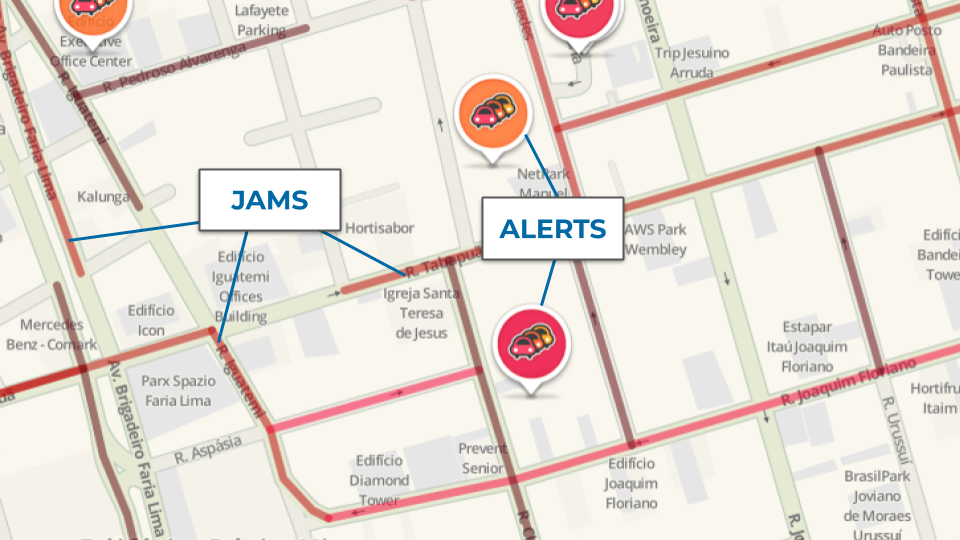
\includegraphics[width=\textwidth]{figures/3-dados-metodologia/from-map-to-data.png}
    \caption{Waze official map with annotations for jams and alerts data. }
    \label{fig:3-waze-map-to-data}
\end{figure}

\begin{sidewaystable}[h]
\begin{tabular}{llll}
\hline
Name & Category & Description & Example \\ \hline
uuid & Identifier & Unique Identifier of the jam & 54515950 \\
pubMillis & Identifier & Milliseconds since 1st of January of 1970 & 1537581410449 \\
country & Geographic & Country name & Brasil \\
city & Geographic & City name & Rio de Janeiro \\
street & Geographic & Street Name & R. Umari \\
level & Traffic Status & \begin{tabular}[c]{@{}l@{}}Current speed percentage of free flow speed.\\0 : 100\% to 80\% of free flow speed  \\1 : 80\% to 61\% of free flow speed \\2 : 60\% to 41\% of free flow speed \\3 : 40\% to 21\% of free flow speed \\4 : 	20\% to 1\% of free flow speed \\5 : blocked road\end{tabular} & 1 \\
delay & Traffic Status & \begin{tabular}[c]{@{}l@{}}Time difference between jam travel time \\ and free flow travel time in seconds\end{tabular} & 12 \\
speed & Traffic Status & Current speed of the road in km/h & 34 \\
line & Traffic Status & \begin{tabular}[c]{@{}l@{}}Array of latitudes and longitudes that describe \\ the segments that are jammed\end{tabular} & \begin{tabular}[c]{@{}l@{}}{[}\{"x": 13.023445, \\"y": -34.5563\}, \{\\"x": 13.02334, \\"y": -34.55234\}{]}\end{tabular} \\
length & Traffic Status & Length of the jam in meters & 23 \\
roadType & Road Characteristics & \begin{tabular}[c]{@{}l@{}}Type of the road code: \\ 1 Streets, 2 Primary Street, \\ 3 Freeways, 4 Ramps, 5 Trails, \\ 6 Primary, 7 Secondary, \\ 8 and 14 4X4 Trails, 9 Walkway, \\ 10 Pedestrian, 11 Exit, \\ 15 Ferry crossing, 16 Stairway, \\ 17 Private road, 18 Railroads, \\ 19 Runway/Taxiway,\\ 20 Parking lot road, 21 Service road.\end{tabular} & 2 \\ \hline
\end{tabular}
\caption{Waze jam data description. Some fields that did not contained relavant information were suppressed.}
\label{table:3-waze-jams}
\end{sidewaystable}

\subsection{Open Street Maps}


Open Street Maps is a open source project that creates and distributes free geographic data. Founded in 2004, the community saw an exponential increase in its early years and has been growing steadily since. In 2019 it reached 5 million unique users that contribute by adding and modifying geographical data (See figure \ref{fig:3-osm-registered-users}). OSM data structure is centered in three basic elements: nodes, ways and relations. Figure \ref{fig:3-osm-features-contributions} shows the creation of those elements over time. There are around 5 billion nodes in 2019, one order of magnitude greater than ways, which had 500 million objects at the same period. This demonstrates that OSM community is already an important source of geographical data.

There is an hierarchy between the elements. The node element is unique and represents a point in the earth surface as a latitude and longitude pair. It can represent standalone features such as ATMs, park benches and others. The way is a ordered collection of elements forming a polygon. This polygon can be open to represent a highway or river. But if the first node is repeated in the end of the collection, the polygon is called closed and it can represent buildings, schools or forests. Finally, the relation documents the relationship between nodes, ways and relations. It can be used to represent a collection of buildings that form an university, an interstate route with several ways and other types of relations. Table \ref{table:3-osm-data} describes the data structure to describe the elements.

Any of those basic elements can carry a tag which gives meaning to it. The tag has two free format fields, key and value in the form \textit{key = value}. For instance, \textit{highway=residential} is a valid tag in which \textit{highway} is the object and  \textit{residential} is the category. Thus, it is a tag for a road that is use to citizens to access their homes. For each element, the key has to be unique, there cannot be a tag \textit{amenity=restaurant} and \textit{amenity=bar}.

Thus, Open Street Maps has important characteristics that motivates its use. It has a large world community that is active and growing. This allows any analysis built upon OSM data to be replicable in other parts of the world. Also, it has a simple and uniform data structure that pinpoints world features in the earth surface and attribute meaning to them.


\begin{sidewaystable}[h]
\begin{tabular}{@{}lll@{}}
\toprule
Name & Description & Example \\ \midrule
id & element unique identifier & 595816010 \\
type & element type: node, way or relation & node \\
tags & \begin{tabular}[c]{@{}l@{}}dictionary of keys and values that gives\\ meaning to the element\end{tabular} & \begin{tabular}[c]{@{}l@{}}\{"highway":"residential",\\ "amenity": "restaurant"\}\end{tabular} \\
lat & geographical coordinate latitude & 51.6825848 \\
lon & geographical coordinate longitude & 3.8384109 \\
nds & \begin{tabular}[c]{@{}l@{}}ordered list of nodes ids that define a polyline.\\ Used in ways.\end{tabular} & \begin{tabular}[c]{@{}l@{}}{[}595816010, 595816013, \\ 595816043{]}\end{tabular} \\
members & ordered list of element ids that define a relation & \begin{tabular}[c]{@{}l@{}}{[}595816023, 595816063, \\ 595816056{]}\end{tabular} \\
changeset & \begin{tabular}[c]{@{}l@{}}changeset number in which the element was created\\ or updated\end{tabular} & 3404386 \\
timestamp & \begin{tabular}[c]{@{}l@{}}date and time in which the element was created\\ or updated\end{tabular} & 2009-12-19 00:42:47.000 \\
uid & \begin{tabular}[c]{@{}l@{}}user unique identifier that created or updated the\\ element\end{tabular} & 195219 \\
user & user name & 3dShapes \\
version & edit version of the element. 1 when newly created & 2 \\ \bottomrule
\end{tabular}
\caption{Open Street Map data description}
\label{table:3-osm-data}
\end{sidewaystable}

\begin{figure}
\centering
\begin{minipage}{\textwidth}
  \centering
  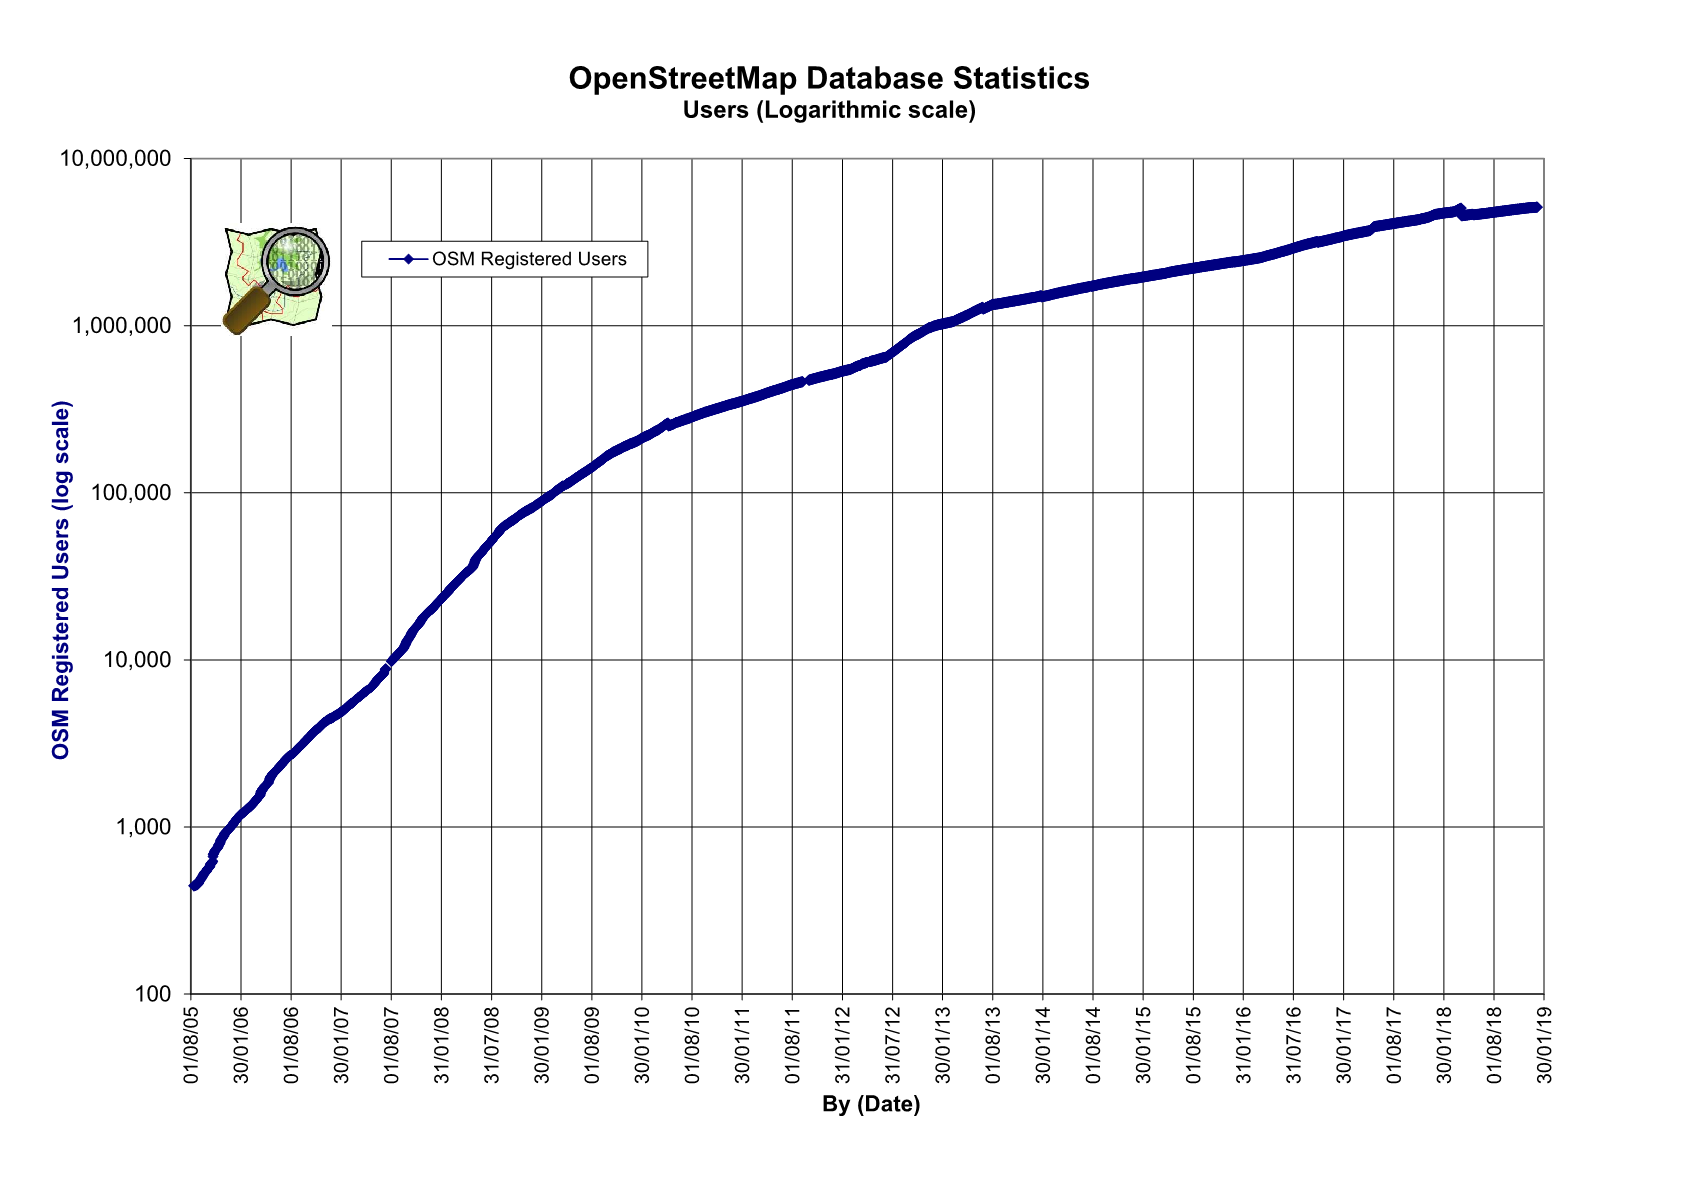
\includegraphics[width=\linewidth]{figures/3-dados-metodologia/osm_registered_users.png}
  \captionof{figure}{Number of unique OSM users over time. The dotted line in blue shows the OSM community is still growing and it has 5 million users that update the map 3 million times a day. Figure from https://wiki.openstreetmap.org/wiki/File:Osmdbstats1_log.png}
  \label{fig:3-osm-registered-users}
\end{minipage}
\begin{minipage}{\textwidth}
  \centering
  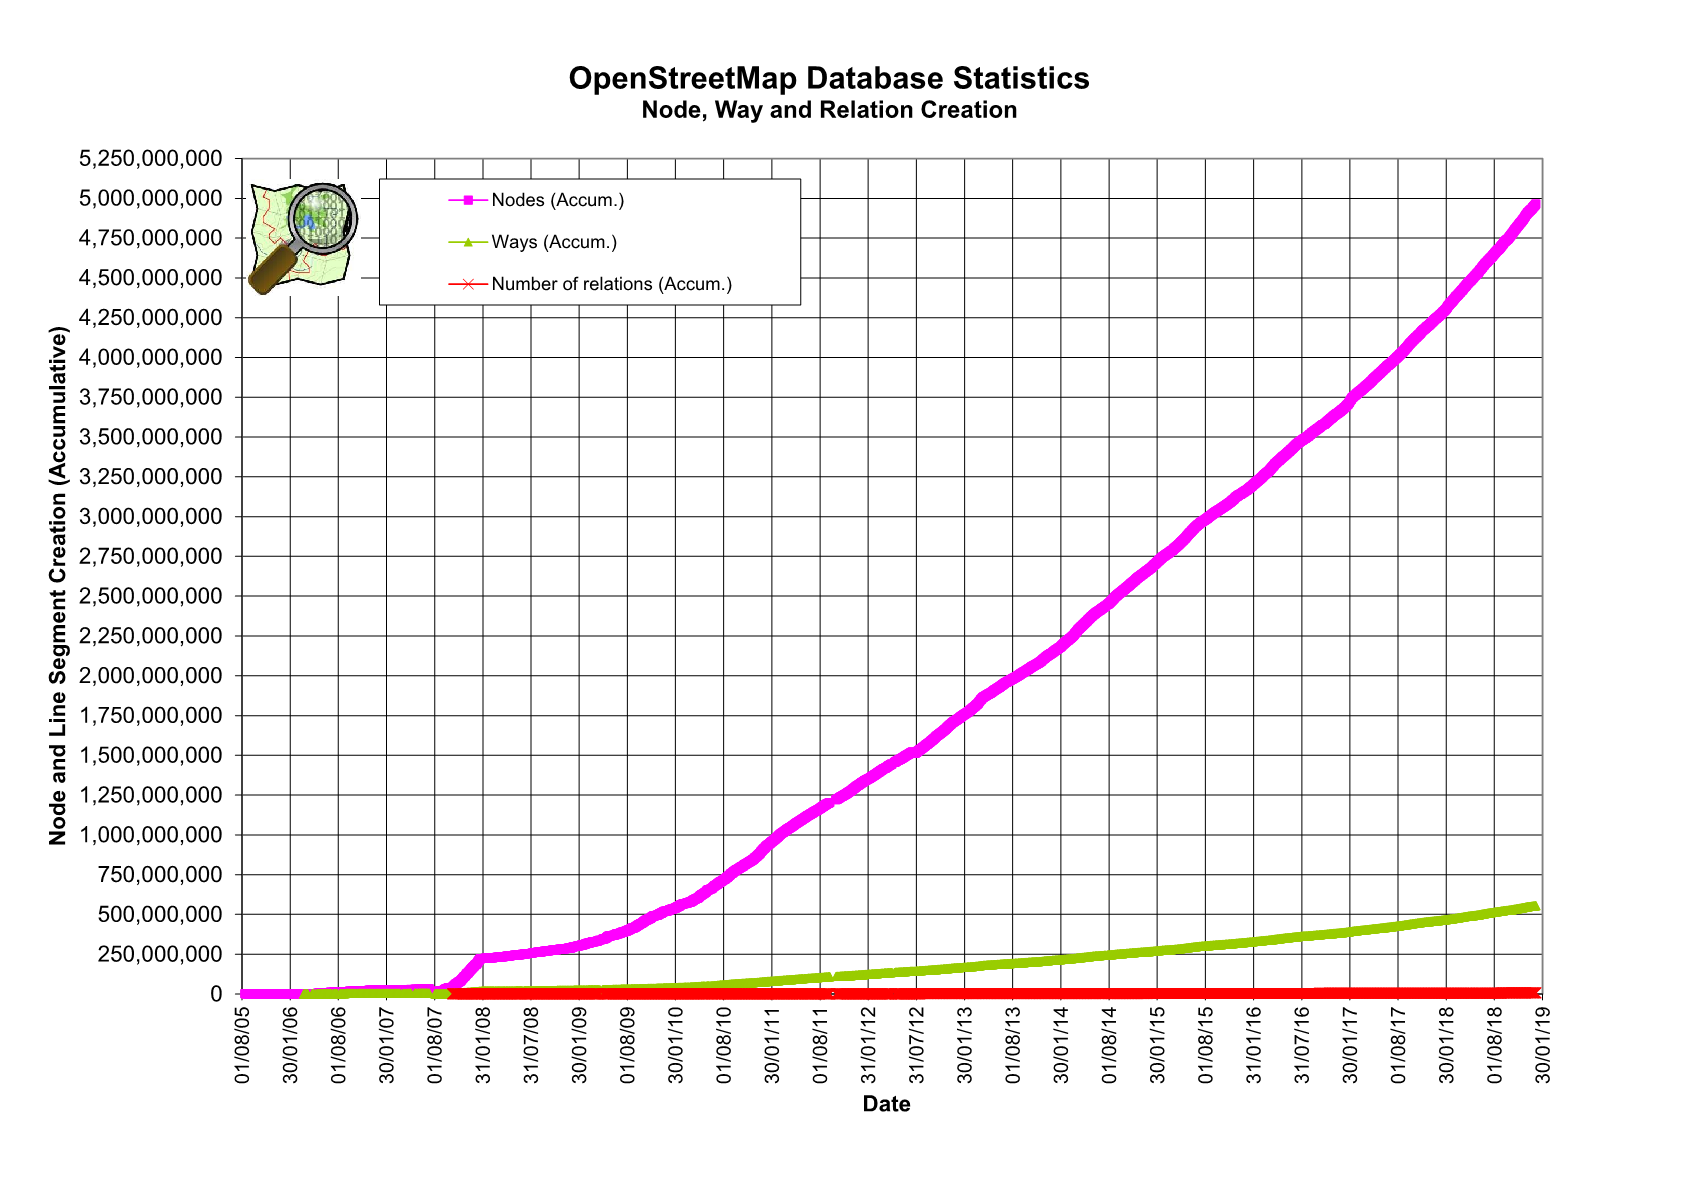
\includegraphics[width=\linewidth]{figures/3-dados-metodologia/osm_features_contibutions.png}
  \captionof{figure}{Evolution of the number of OSM core elements. The nodes, in pink, present a sharp increase since 2007 reaching almost 5 billion objects in January of 2019. Figure from https://wiki.openstreetmap.org/wiki/File:Osmdbstats2.png}
  \label{fig:3-osm-features-contributions}
\end{minipage}
\end{figure}

\subsection{Air Pollution}


The air pollution dataset comes from a Aclima, Inc. and Google project to evaluate fine street air pollution. The companies equipped two cars with 1Hz air pollution measurement devices that sampled for three pollutants: black carbon, NO and NO$_2$. This harmful to health pollutants are emitted by vehicular traffic, shipping, industrial combustion, cooking and heating. The cars drove within residential, industrial and commercial areas of Oakland, California, US, during 1 year. The study emphasized West Oakland (WO) with ~10km$^2$, East Oakland (EO) with ~15km$^2$ and Downtown ~5km$^2$ as seen in Figure \ref{fig:3-pollution-map}, 

The study covered 750 road-km that were divided in 30 m segments. Each segment has on average 31 days and 200 1-Hz measurements data points. Through a process of data reduction and bootstrap resampling algorithms, the researches computed the daytime yearly median and standard error (SE) for ~21.000 road segments. Repeated sampling of the same segment at different seasons and the reduction methods let the researches to obtain stable and precise (\pm10-20\%) estimates of air pollution.

The dataset shared by the researchers has the structure described in Table \ref{table:3-pollution-data-description}. It has the yearly median emission estimates for each road segment and each pollutant, BC, NO and NO$_2$. It is a unique dataset with rich fine grained directed measured data that can be used as a solid basis for statistical inferences.

\begin{figure}[t]
    \centering
    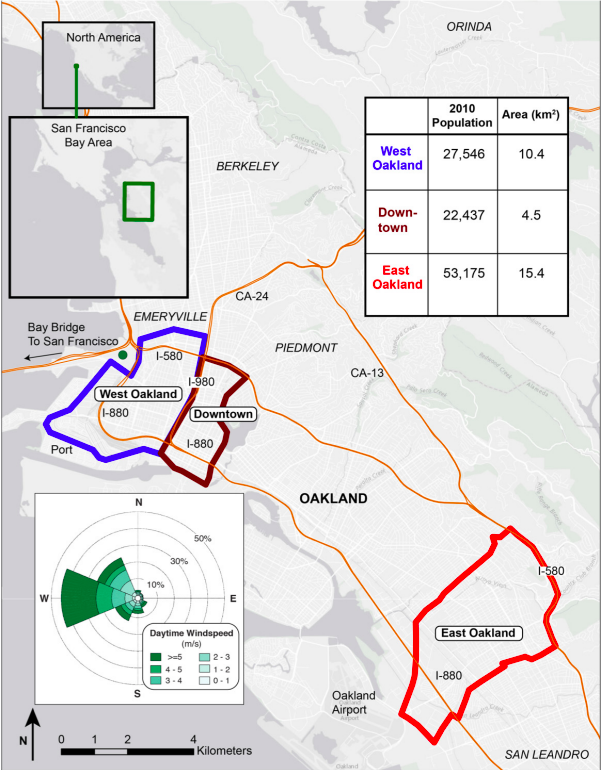
\includegraphics[width=\textwidth]{figures/3-dados-metodologia/pollution-map.png}
    \caption{Areas of Oakland, California, US that were air pollution was estimated by Aclima, Inc and Google. Major highways were annotated and US Census 2010 was used to the population inset. The wind inset shows that at 85\% of daytime the wind was blowing west.}
    \label{fig:3-pollution-map}
\end{figure}

\begin{table}[]
\begin{tabular}{@{}lll@{}}
\toprule
Name & Description & Example \\ \midrule
Lon & \begin{tabular}[c]{@{}l@{}}geographical coordinate longitude of 30 meter \\ segment\end{tabular} & 51.6825848 \\
Lat & \begin{tabular}[c]{@{}l@{}}geographical coordinate longitude of 30 meter \\ segment\end{tabular} & 3.8384109 \\
NO\_Med & \begin{tabular}[c]{@{}l@{}}Median NO concentration for 30 meter road \\ segment in ppm\end{tabular} & 23.4 \\
NO2\_Med & \begin{tabular}[c]{@{}l@{}}Median NO$_2$ concentration for 30 meter road \\ segment in ppm\end{tabular} & 2.5 \\
BC\_Med & \begin{tabular}[c]{@{}l@{}}Median Black Carbon concentration \\ for 30 meter road segment in ppm\end{tabular} & 14.5 \\ \bottomrule
\end{tabular}
\caption{Description of Aclima Inc. and Google data pollution estimate. Parts of the dataset were ommited.}
\label{table:3-pollution-data-description}
\end{table}

\subsection{Uber Hexagons H3}
\begin{itemize}
\item Explain why hexagons
\item Neighbourhood argument
\item H3 Uber grid
\item Advantages: worldwide standard, easy to implement, fast and extensible
\item Picked resolution 9 because it was a size that better balanced granularity and aggregation
\item Image comparing resolutions
\end{itemize}

The estimation presented in this dissertation was not fine grained due to the complexity of factor and lack of relevant features. Thus, we opted to estimate the air pollution density in regions, instead of streets. There are several ways to partition areas of the Earth. It can be a political partition such as neighbourhoods or zip code areas or a geometric shape that repeats over the area of interest. While political partitions are good for day-to-day use to make decision, they irregular geometric structure are subject of to unpredictable change (https://fas.org/sgp/crs/misc/RL33488.pdf). Also, there is no world unified database of political geographical divisions, which turn the task of partitioning the world cumbersome.

We opted to use a regular geometric structure to partition the earth surface. The Uber H3 project already developed an hierarchical hexagon grid for the entire earth surface. 

\begin{figure}[t]
    \centering
    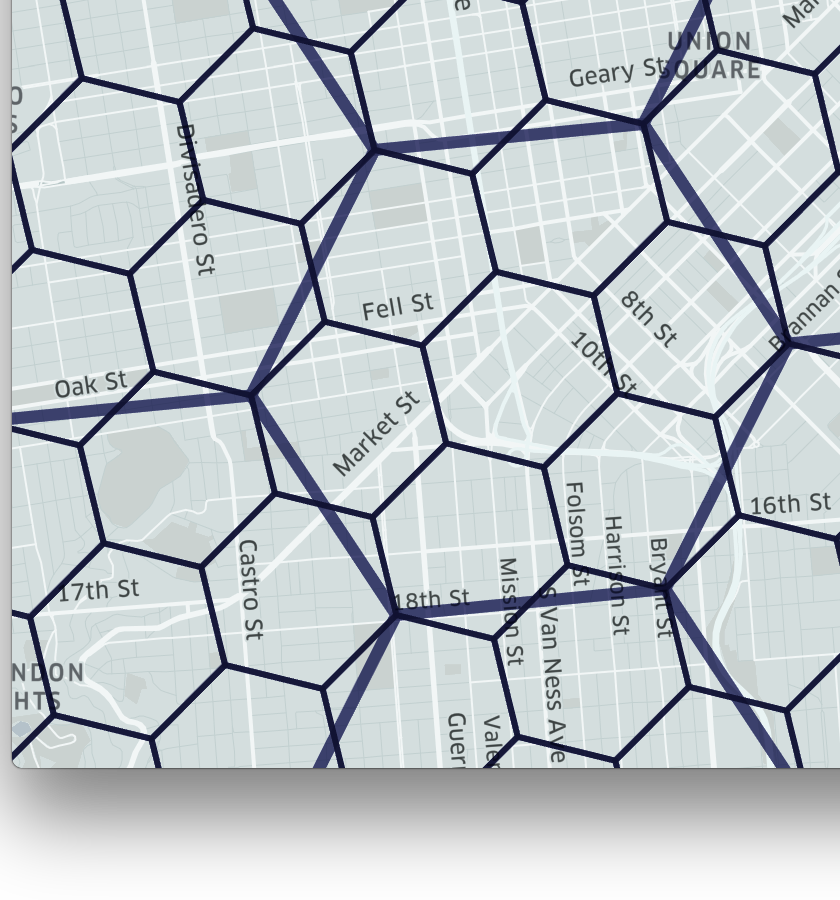
\includegraphics[width=\textwidth]{figures/3-dados-metodologia/h3-hexagons.png}
    \caption{Uber H3 hexagons }
    \label{fig:3-pollution-map}
\end{figure}

\section{Methodology}
\subsection{Features}
\subsubsection{Hexagon Aggregation (H3)}
\begin{itemize}
\item All features were aggregated by H3 hexagons with resolution 9 
\end{itemize}

\subsubsection{Features Waze}
\begin{itemize}
\item Method: simple statistics, max, min, median. 
\item Table with features
\item Point which features were built upon literature references
\item Image of certain features aggregated
\item Table with sample features
\end{itemize}

\subsubsection{Features OSM}
\begin{itemize}
\item Method: Basic count of number of nodes, ways or relations with a tag value with a certain property
\item Table with features
\item Point which features were built upon literature references
\item Image of certain features aggregated
\item Table with sample features
\end{itemize}

\subsubsection{Pollution (Target Variable)}
\begin{itemize}
\item Method: sum of the median of each point
\item Fact: emissions are highly correlated
\item Plot showing correlation and R$^2$ 
\item That is why I chose just NO
\item Image with NO emissions
\end{itemize}

\subsection{Models}
\subsubsection{Linear Regression}

\subsubsection{Spatial Linear Regression }
\subsubsection{Tree Based Model}
\subsection{Car Flee Considerations on Emissions}













